%==========================================================
% Preamble
%==========================================================
% Fonts/languages
\documentclass[english,final,t]{beamer}
\usepackage[orientation=landscape,size=custom,width=129.1,height=86.9,scale=1]{beamerposter}
%\usepackage[T1]{fontenc}
\usepackage[utf8]{inputenc}
%\usepackage{lmodern}          % allows LaTeX to make any arbitrary font size
\usepackage{babel}            % For bibliographies

%\usepackage[scaled]{beramono}  % Load typewriter font first, since Arial doesn't have one
\usepackage{beamerthemePosterExample}

% Beamer Theme
\mode<presentation>
{\usetheme{PosterExample}}
\setbeamertemplate{footline}{}                             % remove footer line
\setbeamercovered{transparent}

% Useful Packages
\usepackage{amsthm}
\usepackage{amssymb}                                               % For fancy math symbols
\usepackage{amsmath}                                               % For awesome equations/equation arrays
\usepackage{mathtools}
\usepackage{float}
\usepackage{prettyref}
\usepackage{graphicx}
\usepackage{enumerate}                                             % For cusomtizable lists
\usepackage{pdflscape}                                             % For landscape-oriented pages
\usepackage{booktabs}
\usepackage{ragged2e}
\usepackage{bm}
\usepackage[most]{tcolorbox}
\usepackage{siunitx}
\usepackage{soul}

%%%%%%%%%%%%%%%% ALGORITHMS  %%%%%%%%%%%%%%%%%%%%%%%%%%%%%%%%%%%%%
\usepackage{algorithm}
\usepackage{algorithmic}
\usepackage[titlenumbered,linesnumbered,ruled,noend,algo2e]{algorithm2e}
% \newcommand\mycommfont[1]{\footnotesize\ttfamily\textcolor{blue}{#1}}
\newcommand\mycommfont[1]{\large \ttfamily\textcolor{blue}{#1}}
\SetCommentSty{mycommfont}
\SetEndCharOfAlgoLine{}
%%%%%%%%%%%%%%%%%%%%%%%%%%%%%%%%%%%%%%%%%%%%%%%%%%%%%%%%%%%%%%%%%%
\newcommand{\bbR}{\mathbb{R}}
\newcommand{\eg}{{\em e.g.,~}}
\newcommand{\cS}{\mathcal{S}}
\newcommand{\cC}{\mathcal{C}}
\DeclareMathOperator{\sign}{sign}
% \usepackage{xcolor}
% \newcommand{\marron}[1]{\textcolor{marron}{#1}}
% \newcommand{\bfmarron}[1]{\textbf{\textcolor{marron}{#1}}}


\robustify\bfseries
\sisetup{
	binary-units            = true,
	tight-spacing           = true,
	separate-uncertainty    = true,
	multi-part-units        = single
}
\usepackage[sort&compress]{natbib}
\bibliographystyle{unsrtnat}

\usepackage{tikz}
%% TIKZ Libraries
\usetikzlibrary{calc,
	decorations,
	patterns,
	shapes,
	arrows.meta,
	decorations.pathmorphing,
	bending,
	math,
	positioning,
	shapes.misc,
	plotmarks,
	fit,
	shadows.blur}
%% TIKZ mark command
\newcommand{\tikzmark}[1]{\tikz[baseline,remember picture] \coordinate (#1) {};}

\DeclarePairedDelimiterX{\norm}[1]{\lVert}{\rVert}{#1}
\DeclareMathOperator*{\argmax}{argmax}
\DeclareMathOperator*{\argmin}{argmin}

\setbeamerfont{title}{size={\fontsize{90}{90}}}
\setbeamerfont{block title}{size={\fontsize{56}{49}}}
\setbeamerfont{block body}{size={\fontsize{36}{42}}}


%% Define colors
\definecolor{bluee}{HTML}{3153ea}
\definecolor{greenn}{HTML}{318e2a}
\definecolor{orangee}{HTML}{b27910}
\definecolor{redd}{HTML}{aa0d0d}

\definecolor{grayy}{HTML}{494949}
\colorlet{inactive}{grayy!60!white}
\definecolor{boxgreen}{HTML}{296b1f}
\definecolor{boxyellow}{HTML}{d8ce38}
\definecolor{boxred}{HTML}{c43a00}
\definecolor{azure}{rgb}{0.0, 0.7, 1}



\newtcolorbox{mybox}{boxrule=6pt,
	colframe=azure}

\newtcolorbox{mybox2}[2][]{colback=malgared!10!white,
	colframe=malgared,fonttitle=\bfseries,
	colbacktitle=malgared,enhanced,
	title=#2,#1}

\title{
	Coordinate descent for SLOPE}
\author{%
\texorpdfstring{
	\begin{minipage}{.98\linewidth}
	\begin{columns}%
		\column{.44\linewidth}
		\centering
		\Large Johan Larsson \\
		\large Lund University, Sweden \\[2em]
		\Large Mathurin Massias \\
		\large Univ. Lyon, Inria, CNRS, ENS de Lyon
		\column{.44\linewidth}
		\centering
		\Large Quentin Klopfenstein \\
		\large Université du Luxembourg \\[2em]
		\centering
		\Large Jonas Wallin \\
		\large Lund University, Sweden
	\end{columns}
	%
	\vspace{1em}
	%
	% \begin{columns}%
	% 	\column{.6\linewidth}
	% 	\centering
	% 	\Large Gauthier Gidel \\
	% 	\large Mila \& Université de Montréal, Canada CIFAR AI Chair
	% 	\column{.4\linewidth}
	% 	\centering
	% 	\Large Mathurin Massias \\
	% \end{columns}
\end{minipage}}{}
}
\setul{0.5ex}{0.3ex}


\DeclareMathOperator{\prox}{prox}
\newcommand{\X}{\mathbf{X}}
\newcommand{\Y}{\mathbf{y}}
\newcommand{\w}{w}
\newcommand{\cL}{\mathcal{L}}
%\setulcolor{red}

%%%%%%%%%%%%%%%%%%%%%%%%%%%%%%%%%%%%%%%%%%%%%%%%%%%%%%%%%%%%%%%%%%%%%%%%%%%%%%%%%%%%%%%%%%%%%%%%%%%%%%%%%%%%
%%%%%%%%%%%%%%%%%%%%%%%%%%%%%%%%%%%%%%%%%%%%%%%%%%%%%%%%%%%%%%%%%%%%%%%%%%%%%%%%%%%%%%%%%%%%%%%%%%%%%%%%%%%%
\begin{document}
\begin{frame}{}
\begin{columns}[t]
%%%%%%%%%%%%%%%%%%%%%%%%%%%%%%%%%%%%%%%%%%%%%%%%%%%%%%%%%%%%%%%%%%%%%%%%
\begin{column}{.3\linewidth}
	\begin{block}{\textbf{\color{malgared} SLOPE and Coordinate descent}}
		\justifying
		SLOPE: a cool sparse penalty with \textbf{\color{malgared}{built-in coefficients clustering}}
		\begin{equation*}
			\mathrm{slope}(\beta) = \sum_{j=1}^p \lambda_j|\beta_{(j)}|
		\end{equation*}
		\vspace{.2em}
		Largest coefficients get penalized more:
		\vspace{.2em}
		\begin{align*}
		&|\beta_{(1)}| \geq |\beta_{(2)}| \geq \cdots \geq |\beta_{(p)}|  \\[5mm]
		& \quad \quad \lambda_1 \geq \ldots \ldots \lambda_p \geq 0
		\end{align*}

		\vspace{.3em}

		\begin{center}
		\includegraphics[width=0.8\linewidth]{./images/slope_level_lines
		}
		\end{center}

		Automatically clusters some coefficients together, better recovery than L1
		\vspace{.4em}

		Issues: not separable, \textbf{\textcolor{malgared}{solvers are slow!}}

	\end{block}
	%
	%
	\begin{block}{\textbf{\color{malgared} Contributions}}
			A new, highly effective solver for SLOPE:
			\vspace{1em}
			\begin{itemize}
				\item  based on \textbf{\color{malgared}hybrid} proximal gradient and coordinate descent
				\item  with \textbf{\color{malgared}guaranteed convergence}
				\item  \textbf{\color{malgared}reduces by orders of magnitude the time}
				 to fit SLOPE
			\end{itemize}
	\end{block}

	% \vspace{1em}
	\begin{block}{\textbf{\color{malgared} Intuition}}

		\begin{center}
			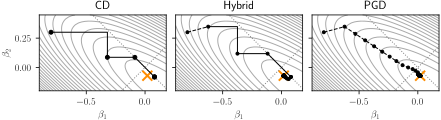
\includegraphics[width=0.8\linewidth]{images/illustration_solvers}

			Naive CD is fast but gets stuck // PGD steps identify the cluster \\[5mm]

			Hybrid: best of both worlds
		\end{center}

	\end{block}
\end{column}
%%%%%%%%%%%%%%%%%%%%%%%%%%%%%%%%%%%%%%%%%%%%%%%%%%%%%%%%%%%%%%%%%%%%
%%%%%%%%%%%%%%%%%%%%%%%%%%%%%%%%%%%%%%%%%%%%%%%%%%%%%%%%%%%%%%%%%%%%
%%%%%%%%%%%%%%%%%%%%%%%%%%%%%%%%%%%%%%%%%%%%%%%%%%%%%%%%%%%%%%%%%%%%
\begin{column}{.3\linewidth}
%%%%%%%%%%%%%%%%%%%%%%%%%%%%%%%%%%%%%%%%%%%%%%%%%%%%%%%%%%%%%%%%%%%%
%%%%%%%%%%%%%%%%%%%%%%%%%%%%%%%%%%%%%%%%%%%%%%%%%%%%%%%%%%%%%%%%%%%%
	\begin{block}{\textbf{\color{malgared}{\#1 Clusterwise minimization}}}
		If we know the clusters of the solution we can find the value of $\beta^*$ on it by solving with CD:
		\begin{equation*}
			\min_{z \in \bbR^{m^*}}\bigg(
				\frac{1}{2} \Big\lVert y - X \sum_{i=1}^{m^*} \sum_{j \in \mathcal{C}_i^*} z_i \sign(\beta_j^*) e_j \Big\rVert^2
				+ \sum_{i=1}^{m^*} | z_i | \sum_{j \in \mathcal{C}_i^*} \lambda_j
				\bigg).
		\end{equation*}

		Idea: allow iterate $\beta$ to \textbf{move only on one cluster} and minimize wrt value on cluster:
		\begin{equation*}
			\beta_i(z) =
			\begin{cases}
			  \mathrm{sign}(\beta_i) z   \, , & \text{if } i \in \mathcal{C}_k \, , \\
			  \beta_i \, ,                    & \text{otherwise} \, .
			\end{cases}
		\end{equation*}

		\textbf{\textcolor{malgared}{Property}}: Minimization with respect to a single clsuter has a closed form given by the \emph{SLOPE-thresholding operator}
		% If we know the true clusters, we need to solve the 1D minimization problem:
		% \begin{equation}
		% 	\min_{z \in \mathbb{R}} \Big(
		% 		G(z) = P(\beta(z))  = \frac{1}{2} \norm{y - X \beta(z)}^2 + H(z)
		% 		\Big) \,  ,
		% \end{equation}
		\end{block}
%%%%%%%%%%%%%%%%%%%%%%%%%%%%%%%%%%%%%%%%%%%%%%%%%%%%%%%%%%%%%%%%%%%%
%%%%%%%%%%%%%%%%%%%%%%%%%%%%%%%%%%%%%%%%%%%%%%%%%%%%%%%%%%%%%%%%%%%%
%%%%%%%%%%%%%%%%%%%%%%%%%%%%%%%%%%%%%%%%%%%%%%%%%%%%%%%%%%%%%%%%%%%%
%%%%%%%%%%%%%%%%%%%%%%%%%%%%%%%%%%%%%%%%%%%%%%%%%%%%%%%%%%%%%%%%%%%%
	\begin{block}{\textbf{\color{malgared}{\# 2 Cluster identification}}}
		%
		{\color{malgared}{Assumptions}}:
		\begin{itemize}
			\item
			$\alpha$-semi convex penalties $g_j / L_j$
			\\
			(common for MCP and SCAD but excludes $\ell_p$, $p<1$)
			\item
			Convergence to a non-degenerated critical point $\hat \beta \in \bbR^p$:\\
			 $\forall j \notin \mathrm{gsupp}(\hat \beta)$,
			$- \nabla f_j (\hat \beta) \in \, \mathrm{int}(\partial g_j(\hat \beta_j))$, with
			$\mathrm{gsupp}(\beta) = \{j \in [p]: \partial g_j(\beta_j) \, \mathrm{is \; a \; singleton}\}$
		\end{itemize}

		 \vspace{0.5em}

		\textbf{\color{malgared}Property}:  Coordinate descent \textbf{identifies the model} in a finite number of iterations: for $\cS = \mathrm{gsupp}(\hat \beta)$, there exists $K>0$ such that for all $k\geq K$, $\beta_{\cS^c}^{(k)} = \hat \beta_{\cS^c}$
		\end{block}
%%%%%%%%%%%%%%%%%%%%%%%%%%%%%%%%%%%%%%%%%%%%%%%%%%%%%%%%%%%%%%%%%%%%
%%%%%%%%%%%%%%%%%%%%%%%%%%%%%%%%%%%%%%%%%%%%%%%%%%%%%%%%%%%%%%%%%%%%
%%%%%%%%%%%%%%%%%%%%%%%%%%%%%%%%%%%%%%%%%%%%%%%%%%%%%%%%%%%%%%%%%%%%
%%%%%%%%%%%%%%%%%%%%%%%%%%%%%%%%%%%%%%%%%%%%%%%%%%%%%%%%%%%%%%%%%%%%
	\begin{block}{\textbf{\color{malgared}{Algorithm}}}

		\begin{algorithm}[H]
			\SetKwInOut{Input}{input}
			\caption{%
			  Hybrid coordinate descent and proximal gradient descent algorithm
			  for SLOPE\label{alg:hybrid}}
			\Input{%
			  \(X \in \mathbb{R}^{n\times p}\),
			  \(y\in \mathbb{R}^n\),
			  \(\lambda \in \{\mathbb{R}^p : \lambda_1 \geq \lambda_2 \geq \cdots > 0\}\),
			  \(v \in \mathbb{N}\),
			  \(\beta \in \mathbb{R}^p\)
			}

			\For{\(t \gets 0,1,\dots\)}{

			  \If{\(t \bmod v = 0\)}{
				\(\beta \leftarrow \prox_{J/{\norm{X}^2_2}}\Big(\beta - \frac{1}{\norm{X}_2^2}X^T(X \beta - y)\Big)\) \label{alg:hybrid-istastep}

				Update \(c\), \(\mathcal{C}\)
			  }
			  \Else{
				\(k \gets 1\)

				\While{\(k \leq \lvert \mathcal{C} \rvert\)}{
				  \(\tilde x_k \gets X_{\mathcal{C}_k} \mathrm{sign}(\beta_{\cC_k}) \)

				  \(z \gets T(c_k\norm{\tilde x}^2 - \tilde x^T(X\beta - y); \norm{x}^2, c^{\setminus k}, \lambda)\)

				  $\beta_{\cC_k} \gets z \mathrm{	sign}(\beta_{\cC_k})$

				  Update \(c\), \(\mathcal{C}\)

				  \(k \gets k + 1\)
				}
			  }
			}
			\Return{\(\beta\)}
		  \end{algorithm}

		\end{block}
	\end{column}
%%%%%%%%%%%%%%%%%%%%%%%%%%%%%%%%%%%%%%%%%%%%%%%%%%%%%%%%%%%%%
%%%%%%%%%%%%%%%%%%%%%%%%%%%%%%%%%%%%%%%%%%%%%%%%%%%%%%%%%%%%%
%%%%%%%%%%%%%%%%%%%%%%%%%%%%%%%%%%%%%%%%%%%%%%%%%%%%%%%%%%%%%
%%%%%%%%%%%%%%%%%%%%%%%%%%%%%%%%%%%%%%%%%%%%%%%%%%%%%%%%%%%%%
	\begin{column}{.3\linewidth}
		\begin{block}{\textbf{\color{malgared}Experimental Results}}
			\setbeamercolor{headerCol}{fg=black,bg=lightgray}
			\begin{center}
					\begin{minipage}{0.9\linewidth}
					\begin{beamerboxesrounded}[lower=headerCol]{}
						\textbf{Code : \url{https://github.com/jolars/slopecd}}
					\end{beamerboxesrounded}
				\end{minipage}
			\end{center}
			%
			\begin{figure}[tb]
				\includegraphics[width=0.7\linewidth]{./images/simulated_legend.pdf}
				\includegraphics[width=0.8\linewidth]{./images/simulated.pdf}

				\textbf{Simulated data}
			\end{figure}
			\vspace{.5em}

			\begin{figure}[tb]
				\includegraphics[width=0.8\linewidth]{./images/real.pdf}

				\textbf{Real data}
			\end{figure}

			References
			\nocite{*}
			\normalsize\bibliography{neuripsBibposter}
		% \end{block}
	\end{block}


	\end{column}
\end{columns}
\end{frame}
\end{document}
